\newpage
\section{A VAR(4) Model of rGDP, rPCE, rGCE, and GPDI}

    We now construct a VAR model to predict GDP, using the general procedure 
    laid out in section \ref{sec:theory}.  Based on some experimentation 
    (omitted here for brevity and time constraints), we choose 3 of the key 
    economic indicators discussed in section \ref{sec:indicators} to include in 
    addition to GDP:
    \begin{itemize}
        \item rPCE (Real Personal Consumption Expenditures)
        \item rGCE (Real Government Consumption Expenditures)
        \item GPDI (Gross Private Domestic Investment)
    \end{itemize}
    
    Our data is drawn from an extensive database of historical
    economic data hosted by the Federal Reserve Bank of St. Louis:
    
    \begin{center} \url{https://research.stlouisfed.org/fred2} \end{center}

    All data is quarterly (3-month) average and already seasonally adjusted.
    We use SAS to perform the actual data analysis and statistical tests.

\subsection{Data Cleaning}
    
    The raw values of our four variables all have strong non-stationary 
    behavior.  Figure \ref{fig:rgdp} shows 50 years of raw GDP data; they
    have a subtly exponential upwards trend.  The other three variables show 
    similar trends.
    
    \begin{figure}
        \begin{center}
        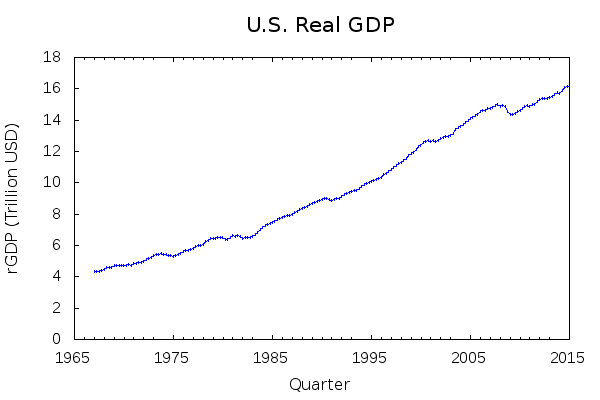
\includegraphics[width=0.9\textwidth]{../img/rgdp.png}
        \end{center}
        \caption{Real U.S. GDP from 1967-2015}
        \label{fig:rgdp}
    \end{figure}
    
    To linearize this trend, we take the log of each variable.  Figure 
    \ref{fig:rgdp-log} shows the results for GDP.  In order to ``de-trend'' the
    data, we then take the first difference of each value as well.  Overall, 
    our preparatory transformation is:
        \begin{equation} \vect{x}'_t = \text{log}(\vect{x}_t) - \text{log}(\vect{x}_{t-1}) \end{equation}
    Figure \ref{fig:rgdp-fdlog} shows the result for GDP.  This procedure 
    provides stationary time series to build our model with, but it also can 
    make the model sensitive to noise in the data (as the first-difference 
    operator tends to magnify noise). Since our indicator data is fairly smooth 
    to begin with, we feel that the choice to use differencing does not 
    adversely affect the model.
        
    \begin{figure}
        \begin{subfigure}{0.5\textwidth}
            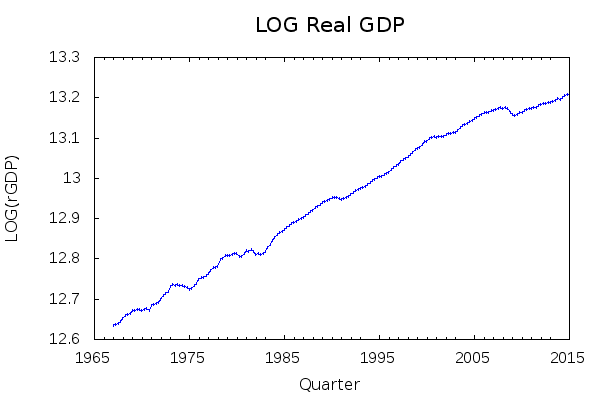
\includegraphics[width=8cm]{../img/rgdp-log.png}
            \caption{Log of U.S. rGDP}
            \label{fig:rgdp-log}
        \end{subfigure}
        \begin{subfigure}{0.5\textwidth}
            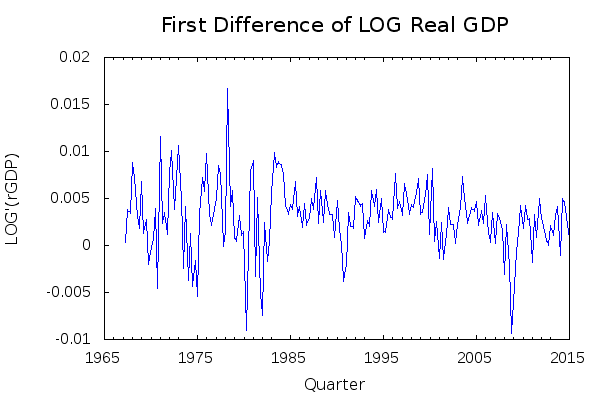
\includegraphics[width=8cm]{../img/rgdp-fdlog.png}
            \caption{First-difference of Log(rGDP)}
            \label{fig:rgdp-fdlog}
        \end{subfigure}
        \caption{Transformed rGDP values.}
    \end{figure}

\subsection{ADF Test Results}
    
    The next step is to test the stationarity of our transformed variables as 
    discussed in section \ref{sec:modelcons}. We construct scalar 
    autoregressive models for order $p \le 2$ for each variable then perform 
    the Augmented Dickey-Fuller test on each.  The results are tabulated in 
    Fig. \ref{fig:adfresults}.  The relevant confidence bounds - Single Mean, 
    Pr $<$ Tau - consistently have $P(\text{unit root}) \le 0.002$.  Thus we 
    confirm that our transformed variables are stationary and suitable for 
    model building.
    
    \begin{figure}[h]
        \begin{subfigure}{0.5\textwidth}
            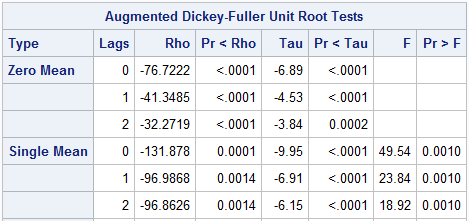
\includegraphics[width=\textwidth]{../img/rgdp-fdlog-ADFtest2.png}
            \caption{(transformed) rGDP}
        \end{subfigure}
        \begin{subfigure}{0.5\textwidth}
            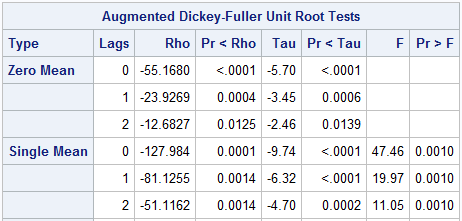
\includegraphics[width=\textwidth]{../img/rpce-fdlog-ADFtest2.png}
            \caption{(transformed) rPCE}
        \end{subfigure}
        \begin{subfigure}{0.5\textwidth}
            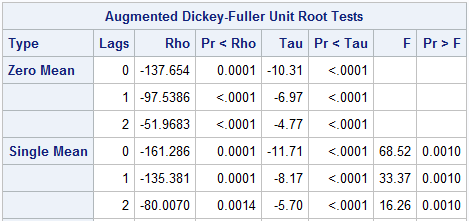
\includegraphics[width=\textwidth]{../img/rgce-fdlog-ADFtest2.png}
            \caption{(transformed) rGCE}
        \end{subfigure}
        \begin{subfigure}{0.5\textwidth}
            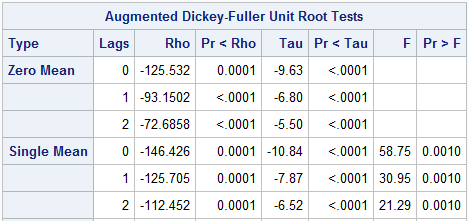
\includegraphics[width=\textwidth]{../img/gpdi-fdlog-ADFtest2.png}
            \caption{(transformed) GDPI}
        \end{subfigure}
        \caption{Augmented Dickey-Fuller test results for selected, transformed indicator variables.}
        \label{fig:adfresults}
    \end{figure}

\subsection{AIC Results}

    With our individual variable transformations validated, we can begin comparing
    candidate VAR models.  We build models for orders $1 \le p \le 6$ and compare them
    using the AIC measure as discussed in section \ref{sec:modelorder}.
    
    The results are tabulated in Tab. \ref{tab:aicresults}.  They suggest that
    the optimal order is $p = 4$, and we choose to proceed with a VAR(4) model.
    It is worth noting that a time lag of 4 quarters seems natural: the economy
    is well known to go through annual cycles, and despite the fact that the raw
    data is seasonally adjusted it is likely that some traces of those cycles remain.
    \begin{table}[h]
    \begin{center}
    \begin{tabular}{|c|r|r|r|r|r|r|}
        \hline $p$ & 1 & 2 & 3 & \cellcolor{lightgray}\color{blue}4 & 5 & 6 \\
        \hline AIC & -44.9464 & -44.9059 & -44.9927 & \cellcolor{lightgray}\color{blue}-45.0499 & -44.9380 & -38.5330 \\
        \hline
    \end{tabular}
    \end{center}
    \caption{Akaike Information Criterion results for VAR models up to order 6.}
    \label{tab:aicresults}
    \end{table}

\subsection{Model Fitting} 

    Using the method of ordinary least-squares, we determine the coefficients
    for our VAR(4) model:    
    \begin{align*}
        log(rGDP)_t =  0.0002 
        + \left( -0.332, -0.191, -0.402, -1.314 \right) \cdot \vect{x}_{t-1} \\
        + \left(  0.005,  0.045, -0.135,  0.450 \right) \cdot \vect{x}_{t-2} \\
        + \left(  0.051, -0.430, -0.047,  0.570 \right) \cdot \vect{x}_{t-3} \\
        + \left(  0.195, -0.188,  0.225,  0.912 \right) \cdot \vect{x}_{t-4}
    \end{align*}
    \[ \text{with } \vect{x} = \begin{pmatrix} log(rGDP) \\ log(rPCE) \\ log(rGCE) \\ log(GPDI) \end{pmatrix} \]

    The model diagnostics show significance and low RMS residuals: 
        \[ (Pr>f) \le .0001 \]
        \[ \sigma_\text{res\_gdp} = .00301 \]  
    Overall, the model is an excellent fit for all the raw data, although we are
    mostly interested in the GDP values.
    A plot of the model "predictions" of historical GDP is shown in Fig. \ref{fig:fitoverlay}.
        
    \begin{figure}
        \begin{center}
        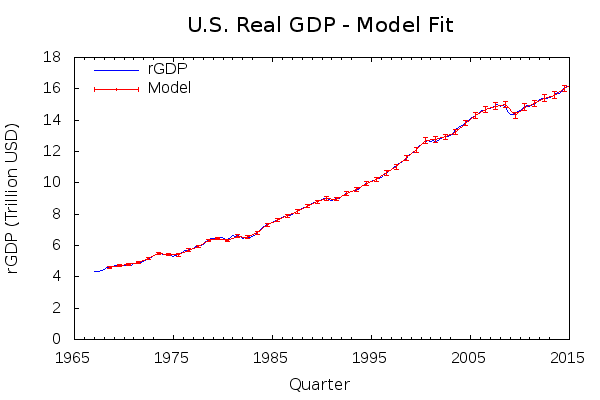
\includegraphics[width=0.75\textwidth]{../img/model1-rgdp-fit.png}
        \end{center}
        \caption{U.S. GDP vs. model predictions}
        \label{fig:fitoverlay}
    \end{figure}
    
    \begin{figure}[!h]
        \begin{subfigure}{0.5\textwidth}
            \begin{center}
            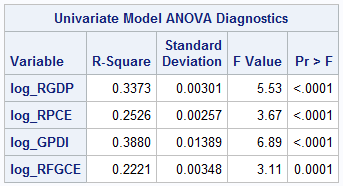
\includegraphics[width=\textwidth]{../img/model1-fitstats.png}
            \end{center}
            \caption{Statistical measures of model fit}
        \end{subfigure}
        \begin{subfigure}{0.5\textwidth}
            \begin{center}
            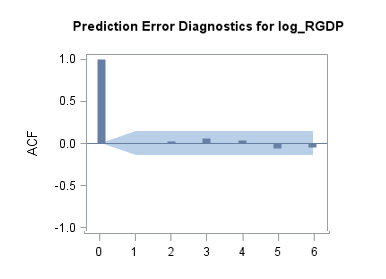
\includegraphics[width=\textwidth]{../img/model1-residualdiagnostics.png}
            \end{center}
            \caption{Autocovariance distributions of GDP residuals}
            \label{fig:residualdiag}
        \end{subfigure}
        \caption{}
    \end{figure}

    We also examine the autocovariance of the residual error.  In Eq. \ref{eq:stochastic3},
    we state that the autocovariance of the stochastic term in an AR model must
    be zero for all time lags $T > 0$.  Figure \ref{fig:residualdiag} shows that
    this is also notably true of our residual errors.  This supports our implicit
    assumption that GDP can, in fact, be modeled with VAR.
    